\documentclass[10pt]{article}

\usepackage[margin=1.5in]{geometry}
\usepackage{graphicx}
\usepackage{natbib}
%correct punctuation for MBE
\bibpunct[,]{(}{)}{;}{a}{}{,}
\usepackage{tablefootnote}
\usepackage{amsmath}

\renewcommand{\bottomfraction}{.9}
\renewcommand{\topfraction}{.9}
\renewcommand{\textfraction}{0.1}
\renewcommand{\floatpagefraction}{.9}

\linespread{1.1}
\begin{document}

\title{\textbf{(working title) Filtering with Guidance is pretty useless}}
\author{Stephanie J. Spielman$^{1*}$ and Eric T. Dawson$^{1}$ Claus O. Wilke$^{1}$}
\date{}

\maketitle
\noindent
Address:\\
$^1$Section of Integrative Biology and Center for Computational Biology and Bioinformatics. The University
of Texas at Austin, Austin, TX 78731, USA.\\

\bigskip
\noindent
$^*$Corresponding author\\
$\phantom{^*}$Email: stephanie.spielman@utexas.edu\\

\bigskip
\noindent
Manuscript type: research article

\bigskip
\noindent Keywords: multiple sequence alignment, alignment filters, sequence simulation, positive selection inference

\newpage
\begin{abstract}
	Most nucleotide or amino acid sequence studies begin with building a multiple sequence alignment (MSA) with the goal of assigning homology across positions of these diverged sequences. Although a critical step in nearly sequence evolution studies, MSAs may represent a substantial source of error in subsequent applications, ranging from phylogenetic reconstruction to evolutionary rate inference. Motivated by this issue, many have suggested methods which can identify putatively poorly aligned regions in MSAs so that researchers can remove these regions from analyses in an effort to reduce error. One recent method, known as Guidance, generates position-based confidence scores in a given MSA using a bootstrap approach. Some studies have suggested that applying a Guidance filter to protein-coding sequence alignments can improve accuracy in positive selection inference. However, the specific circumstances under which Guidance might offer improvements remain unclear. To elucidate how the Guidance filter behaves in realistic protein-coding sequences, we have re-implemented the Guidance software with several statistical improvements, including methods to phylogenetically correct confidence scores. We find that, overall, neither the original Guidance nor our phylogenetically-corrected version substantially improves positive selection inference. Thus, we cannot equivocally advocate the use of a Guidance-based filter for positive selection inference.
\end{abstract}


\section*{Introduction}
Constructing a multiple sequence alignment (MSA) represents the first step of analysis in most studies of molecular evolution, namely phylogenetic reconstruction and evolutionary rate inference. Recently, several studies have shown that poor MSA quality can significantly hinder accuracy in such downstream analyses \citep{Jordan2011, MarkovaRaina2011, Dwivedi2009, Talavera2007, Ogden2006}. In particular, using low-quality MSAs during positive selection inference tends to yield elevated false positive rates \citep{Jordan2011, Privman2012, Schneider2009, Fletcher2010}. As a consequence, many have advocated applying an alignment filter to MSAs before their use in such analyses. Such filters, which include Guidance \citep{Penn2010, Privman2012}, GBLOCKS \citep{Castresana2000} and T-Coffee \citep{Notredame2000}, locate putatively poorly aligned regions in alignments, thereby allowing users to curate their alignments to maximize signal. The hope is that culling unreliable positions and/or columns from MSAs will yield increased accuracy in positive selection inference, without excessively sacrificing power.

Of these filters, Guidance \citep{Penn2010} is currently the most widely used in positive selection inference. Guidance derives a confidence score for each MSA position using a bootstrap approach that samples variants in a progressive alignment guide tree. Using the resulting confidence scores, users can ``mask" (i.e. replace with an ambiguous character such as ``?" or ``N") positions which score below a given threshold, thereby removing residues that cannot be confidently placed in the alignment. This method is fairly conservative, as particular positions of low confidence can be removed rather than entire columns. Moreover, recent simulation studies have demonstrated that filtering poorly aligned residues with Guidance may confer increased accuracy when inferring positive selection \citep{Jordan2011,Privman2012}. 

Even so, while Privman et al. \citep{Privman2012} found dramatic improvements in positive selection inference when applying the Guidance filter, Jordan and Goldman's \citep{Jordan2011} comprehensive study on alignment methods and filtering found that Guidance yields modest, if any, effects on this inference. In particular, they reported that, at typical protein divergence levels or insertion/deletion (indel) rates, Guidance offers few benefits to positive selection inference; while the Guidance filter did not obscure signal, neither did it improve inferences. Alternatively, at extremely high divergence levels (1.8 mean path length, defined as mean root-to-tip branch length) or indel rates (0.2 indel/substitution events), Jordan and Goldman found that Guidance significantly boosted true positive rates. While these results were compelling, protein sequences used in positive selection studies, however, rarely, if ever, contain sequences separated by such high divergences; for example, a typical mammalian gene tree's MPL is only about 0.17 \citep{Spielman2013}, 10\% the divergence level at which Jordan and Goldman detected improvements when using the Guidance filter.

Motivated by these apparent discrepancies, we sought to determine whether altering the Guidance scoring algorithm could yield improved inferences at more realistic divergence and/or indel levels. To this end, we re-implemented the Guidance software (see Methods for details) and examined the effects of new scoring algorithms which take the sequences' phylogenetic relationships into account. We simulated sequences according to realistic evolutionary parameters along real gene trees, and conducted alignments using this re-implementation. We inferred evolutionary rates using both the recently-described method Fubar \citep{Murrell2013} and the widely-used Paml M8 model \citep{Yang2007}. Overall, we found that neither the original Guidance filter nor our newly implemented filters confer any significant benefits to positive selection inference. In fact, for alignments with fewer sequences, applying these filters may obscure signal to the point where positive selection inference worsened relative to an unfiltered alignment. In cases where these filters did yield improvements, the magnitude of the benefit was minimal (at most, a 3\% increase in true positive rates). Thus, we cannot unequivocally advocate the use of such filters when inferring positive selection in protein-coding sequences.


\section*{Results}

\subsection*{Guidance re-implementation and analysis pipeline}
To systematically evaluate Guidance`s influence on positive selection inference, we re-implemented the Guidance software in python and C++. Before conducting any analyses, we verified that, given a set of perturbed alignments, our program produced the same position scores as the original Guidance. In addition to our basic Guidance re-implementation, we derived two new algorithms which employ phylogenetic weighting when assigning confidence scores (see Methods for details).  Briefly, the first method incorporated a weight for each sequence in the alignment, as calculated by BranchManager \citep{Stone2007}, and the second method incorporated patristic distances (the sum of branch lengths between two taxa). We called these methods, respectively, BMweights and PDweights.  We additionally proposed a ``gap-penalization” score normalization scheme, which naturally assigned lower confidence scores to residues in highly gapped regions, given that such regions were more likely to be poorly aligned. We referred to filters using the gap-penalization scheme as GuidanceP, BMweightsP, and PDweightsP.

Figure~\ref{pipeline} shows the overall pipeline for our analysis. First, we simulated realistic protein-coding sequences using Indelible \citep{Fletcher2009} along four different gene trees of sizes 11, 26, 60, and 158 taxa. To ensure that these simulations produced real sequence data to the extent possible, we simulated according to evolutionary parameters inferred from H1N1 influenza hemagluttinin (HA), a protein well known to contain positively selected regions \citep{Meyer2012}. We then processed the unaligned sequences with our Guidance re-implementation using the aligner mafft L-INS-I (linsi) \citep{Katoh2005}. We chose to use only linsi, which strongly outperforms other similar alignment softwares for protein alignments \citep{Thompson2011,Nuin2006}without sacrificing speed. We scored each alignment using each of our three scoring algorithms (original Guidance, BMweights, and PDweights) with each of our two normalization schemes (original Guidance and gap-penalization), representing a total of six filtering conditions per alignment. We masked residues whose score was below $0.5$ with ``?".  

Finally, we inferred evolutionary rates with both the recently-described Fubar \citep{Murrell2013} and Paml's M8 model \citep{Yang2007}. We considered sites as inferred to be positively selected if the given method returned a posterior probability $\geq0.9$. Note that, while we processed all alignments with Fubar, we did not infer positive selection for the largest simulation set with Paml due to prohibitive runtimes. 


\subsection*{Filtering with Guidance has limited utility}

We assessed how filtering alignments with a Guidance-based method influences positive selection detection by comparing the resulting true positive rate (TPR) of positive selection inference between all filtered alignments and their corresponding unfiltered alignments. To this end, we build mixed-effects linear models for each sequence simulation set, with the simulation count as the random effect to account for the paired structure of our analysis (as in, each alignment was filtered with multiple strategies, rendering them dependent), for Fubar and Paml separately. 
We chose to primarily compare TPRs among alignments as the false positive rates (FPR) were exceedingly small, mostly between $0-10^{-2}$ on average across simulation sets and methods. These rates were similar to those recovered by \citep{Jordan2011}, and we attribute their low magnitudes to being artifacts of sequence simulation. \textbf{We do not, however, have any idea how the Guidance paper found FPR around 20\%. That result we attribute to a fundamental misunderstanding of how to calculate FPR. <--- obviously I won't say this, but should I say something that gets this across but in a PC way? Or only if a reviewer gets angsty?}

We first compared the two normalization schemes to one another using mixed effects models with TPR as the response variable, simulation count as a random effect, and normalization scheme as a fixed effect. Only filtered alignments were considered in these models, results from which are seen in Table~\ref{penalmodel}. In all instances in which we detected significant difference between normalization schemes, the gap-penalization scheme outperformed the original Guidance scheme, albeit by very small magnitudes. Even so, as the gap-penalization method yielded marginally better performance in positive selection inference. Therefore, we proceeded to compare the results from gap-penalization algorithms (GuidanceP, BMweightsP, PDweightsP) to those of unfiltered alignments with a second series of mixed-effects models. These models included TPR as the response variable, simulation count as a random effect, and algorithm as a fixed effect. Table~\ref{casemodel} gives the results from these models for each simulation set and selection inference method.

Overall, we did not recover any difference in TPR among gap-penalization filtering algorithms; Guidance and the two phylogenetically-weighted methods performed statistically indistinguishably for a given simulation set. When processed with Fubar, alignment filtering significantly increased TPRs for the 60 and 158-sequence simulation sets, but neither improved nor worsened positive selection inference for the 11 or 26-sequence simulation sets. Even so, the magnitude of its improvements were relatively small, boosting unfiltered TPRs by an average of 0.03 for the 60-sequence set and by 0.01 for the 158-sequence set. 
Results from Paml did not result in a significant change in TPR for the 11 or 60-sequence simulation sets, but filtering did improve TPRs in the 26-sequence simulation set by roughly 0.009. Thus, while we did detect some benefits to filtering with a Guidance-based method, the magnitudes of these effects were relatively insubstantial.

As the results from our models were highly sensitive to the posterior probability chosen when assigning sites as positively selected, we visually assessed how selecting a different posterior probability threshold would influence filtering. Figure ~\ref{tprfpr} shows, for unfiltered alignments, how this threshold influences TPR and FPR for both Fubar and Paml, averaged across results from the 60-sequence simulation set.
\textbf{Paml demonstrated weird behavior that I don't really know how to describe for its TPR.} Interestingly, Paml's FPR dropped to nearly zero even at the lowest posterior probability threshold, where as Fubar shows a smoother curve downwards, reaching a zero FPR above 0.8. This difference likely reflects the different approaches the methods adopt; Paml's M8 model aims to identify precise $dN/dS$ value at each site in an alignment, whereas Fubar merely approximates whether a site is positively selected but does not attempt to assign a point estimate of $dN/dS$ to each position. This behavior has some implications for alignment filters, as well, as seen in Figure ~\ref{smalltpr}, which shows TPR for both Fubar and Paml at posterior probability cutoffs that a typical study would employ. The filtered alignments, as processed with Fubar, were clearly above the unfiltered alignment line, whereas, when processed with Paml, they were indistinguishable from the unfiltered alignment. \textbf{but this is the same as the model!}.

We conducted an ROC analysis to broadly compare accuracy across filters and between Fubar and Paml (Figure~\ref{roc}). However, while useful in assessing theoretical performance, it would be difficult to recover results comparable to these ROC curves in real analyses. FPR and TPR recovered in real analyses depend more precisely















\section*{Discussion}

\textbf{all of this is old, probably written early December}.
Our comprehensive study of alignment filtering with Guidance-based methods indicated that, while masking individual sites rarely hinders positive selection inference, neither does it significantly improve inferences when analyzing protein sequences at realistic divergence levels. These results mirror those made by Jordan and Goldman`s \citep{Jordan2011} study on alignment methods and filtering. That the weighted algorithms are unable to improve upon the original Guidance algorithm may indicate the minimal benefits that filtering in this manner produces at all. Were Guidance to offer robust improvements when detecting positively selected sites, one might expect that the more statistically controlled approach would boost the method`s performance. However, as we have found that the method itself does not dramatically, if at all, influence positive selection inferences, it is not entirely unexpected that improving the algorithm does not help, either. Based on our results, then, we cannot unequivocally recommend filtering alignments in the manner presented here. 

\section*{Methods}

\subsection*{Guidance Reimplementation}
Our reimplemented Guidance is written in Python and C++. Following the algorithm set forth in Penn et al. \citep{Penn2010}, we first create a reference amino-acid alignment using a user-specified progressive alignment software, with choices of clustalw \citep{Thompson1994}, muscle \citep{Edgar2004}, or mafft \citep{Katoh2002, Katoh2005}. For our analysis, we used only mafft L-INS-I (linsi) for all alignments. We then generate 100 bootstrapped alignment replicates, each of which is used to create a bootstrapped tree in FastTree2 \citep{Price2010}. We then use these 100 trees as “guide trees” in creating 100 new “perturbed” alignments, which are subsequently compared to the reference alignment to generate a Guidance score for each residue.

\subsection*{Scoring Algorithms}
In addition to this basic re-implementation, we implemented two additional scoring algorithms which incorporating phylogenetic information. Before calculating scores, we create a phylogeny using the reference alignment. Our program includes functionality for several maximum likelihood phylogenetic softwares, including FastTree2 \citep{Price2010} and RAxML \citep{Stamatakis2006}. Using this phylogeny, we can calculate two types of phylogenetic weights. The first uses the software package BranchManager \citep{Stone2007} to calculate a weight for each taxon in the phylogeny representing that taxon's contribution to the phylogeny as a whole. We call this method ``BMweights." The second method calculates patristic distances between each taxon in the phylogeny using the python package DendroPy \citep{Sukumaran2010}. We call this method ``PDweights."


We calculated positional confidence scores for each of the $n$ bootstrap alignment as follows. A raw score, $S$, for a given residue in column $j$, row $i$ of the reference alignment is calculated as \begin{equation} S_{ij} = \sum\limits_{}^k s_{ik}^j I_{ik}^j\end{equation}, where $k$ represents all rows in column $j$ which are not gaps. 
In this formula, the indicator function 
\begin{equation}I_{ik}^j = \left\{ \begin{array}{rl}

              1                         &\mbox{if reference alignment residue pair (i,k) is present in bootstrap alignment} \\
              0            &\mbox{if reference alignment residue pair (i,k) is absent in bootstrap alignment} \\
                     \end{array} \right. 
\end{equation}
served to compare the bootstrap and reference alignment residue pairings.
We calculated $s_{ik}^j$ based on the given scoring algorithm:

\begin{equation}
s_{ik}^j = \left\{ \begin{array}{rl}

              1                         &\mbox{if Guidance} \\
              w_iw_k              &\mbox{if BMweights} \\
              d_p(i,k)              &\mbox{if PDweights} \\
                     \end{array} \right.,
\end{equation}

where $w_i$ was the phylogenetic weight of the taxon at row $i$, as calculated by BranchManager, and $d_p(k,i)$ was the patristic distance (sum of branch lengths) between the taxa at rows $i$ and $k$. 

We then summed positional scores $S_{ij}$ determined from each bootstrap alignment. Scores were normalized to yield a final score $\widetilde{S}_{ij}$ at each residue in the reference alignment using two different schemes. The first scheme, given by \begin{equation} \widetilde{S}_{ij} = \frac{S_{ij}}{n\sum\limits_{}^k S_{kj}}, \end{equation} normalized by only considering the residue-residue comparisons made, as done by \citep{Penn2010}. The second scheme was given by 

\begin{equation} \widetilde{S}_{ij} = S_{ij} \bigg/ \left\{ \begin{array}{rl}
              n\times (l-1)                                   &\mbox{if Guidance} \\
              n\sum d_p(i,l)                         &\mbox{if BMweights} \\
   		  nw_i                                       &\mbox{if PDweights} \\          
         \end{array} \right.,
\end{equation}
where $l$ represented all rows (including gaps) in column $j$ \textbf{l is used in two diff ways in the above formula. need better representation!}. This second normalization scheme inherently gave lower scores to highly gapped columns, and we therefore called it the ``gap-penalization" normalization.

Thus, in total, we used our Guidance re-implementation to test six different masking algorithms: the original Guidance, weighting using BranchManager weights, and weighting using patristic distance, with two normalization schemes each. We refer to these algorithms as Guidance, BMweights, and PDweights, with their respective gap-penalized versions called GuidanceP, BMweightsP, and PDweightsP.



\subsection*{Sequence Simulation}
Coding sequences were simulated using Indelible \citep{Fletcher2009}. To ensure that our simulations reflect realistic protein sequences, we simulated according to evolutionary parameters of the H1N1 hemagluttinin (HA) influenza protein. To derive these parameters, we aligned 1028 HA protein sequences in mafft linsi \citep{Katoh2005} of 1038 HA amino acid sequences, and then back-translated to a codon alignment using the original nucleotide sequence data. We generated a phylogeny from this codon alignment in RAxML \citep{Stamatakis2006} using the ``GTRGAMMA" model. Using the codon alignment and phylogeny, we inferred evolutionary parameters with the REL (random effects likelihood)  method \citep{NielsenYang1998} using the software HyPhy \citep{Pond2005}, with five evolutionary rate categories as free parameters under the GY94 evolutionary model \citep{GoldmanYang1994}. We employed a Bayes Empirical Bayes approach \citep{Yang2000} to obtain infer $dN/dS$ values at each site, which we used to assess a complete distribution of site rates. The resulting distribution was log-normal with a mean $dN/dS = 0.37$ with and 8.3\% of sites were under positive selection. We binned these rates into 50 equally spaced categories for specification in Indelible, which requires a discrete distribution of $dN/dS$ values. Again according to parameters derived from the HA analysis, kappa was fixed at 5.3 for all simulations. We additionally set the state codon frequencies for our simulations according to those directly calculated from HA alignment. 

To simulate across different numbers of taxa, we simulated 100 alignments across four different real gene trees each, yielding a total of 400 simulated alignments. Phylogenies used included an 11-taxon tree of the mammalian olfactory receptor OR5AP2 \citep{Spielman2013}, a 26-taxon tree of mammalian rhodopsin sequences\citep{Spielman2013}, a 60-sequence tree of phosphoribulokinase (PRK) genes from photosynthetic eukaryotes \citep{Yang2011}, and a 158-taxon multilocus tree of flatfish sequences \citep{Betancur2013}.
For each simulation set, we directly calculated an indel (insertion-deletion) rates directly from these trees’ original alignments, to use as simulation parameters, by dividing the total number of gaps present by the total number of positions in each alignment. Respectively, indel rates were 0.053, 0.019, 0.0041, and 0.0066. 

\subsection*{Alignment and Positive Selection Inference}
Alignments were built with mafft linsi \citep{Katoh2002,Katoh2005}. Using our re-implemented Guidance software, we generated 6 filtered alignments (one for each filtering algorithm), masking residues with scores below cutoff of 0.5. We infered positive selection for every condition using both the recently-described software Fubar \citep{Murrell2013} and the widely-used Paml M8 model \citep{Yang2007}. We used the scoring tree, built during the Guidance alignment procedure, as the input phylogeny for selection inference. Therefore, all alignments derived from the same base sequence were processed with identical phylogenies to remove any potential bias. Note that while we employed Fubar to assess positive selection for all simulation sets, we did not use Paml to infer positive selection for the largest set (158 sequences).

We then compared resulting positive selection inferences for each alignment to its respective true alignment's $dN/dS$ values, given by Indelible during simulation, to assess performance accuracy. As residues may be differently aligned relative to the true simulated alignment, we adopted a consensus method to compare evolutionary rates. In other words, to compare evolutionary rates between between true and inferred alignments, we required that at least 50\% of the residues present in a true alignment column be present in an inferred alignment column. If this condition was met, we considered the true alignment column’s $dN/dS$  selection status (negative, neutral, or positive) to be the true value for the given inferred column. To assign sites as positively selected, we adopted different posterior probability cutoffs for each simulation set based on the inference method, as Fubar and Paml have different levels of accuracy. We identified the posterior probability threshold for each simulation set such that the resulting average false positive rate in unfiltered alignments was 1\%. The posterior probability cutoffs used are seen in Supplementary ~\ref{postprob}.

Statistics were performed using in-house python and R scripts. Linear modeling was conducted using the R packages lme4 \citep{Bates2012} and
multcomp \citep{Hothorn2008}. All code used is available at \textbf{the github or something}.


%\begin{figure*}[H]
%\centerline{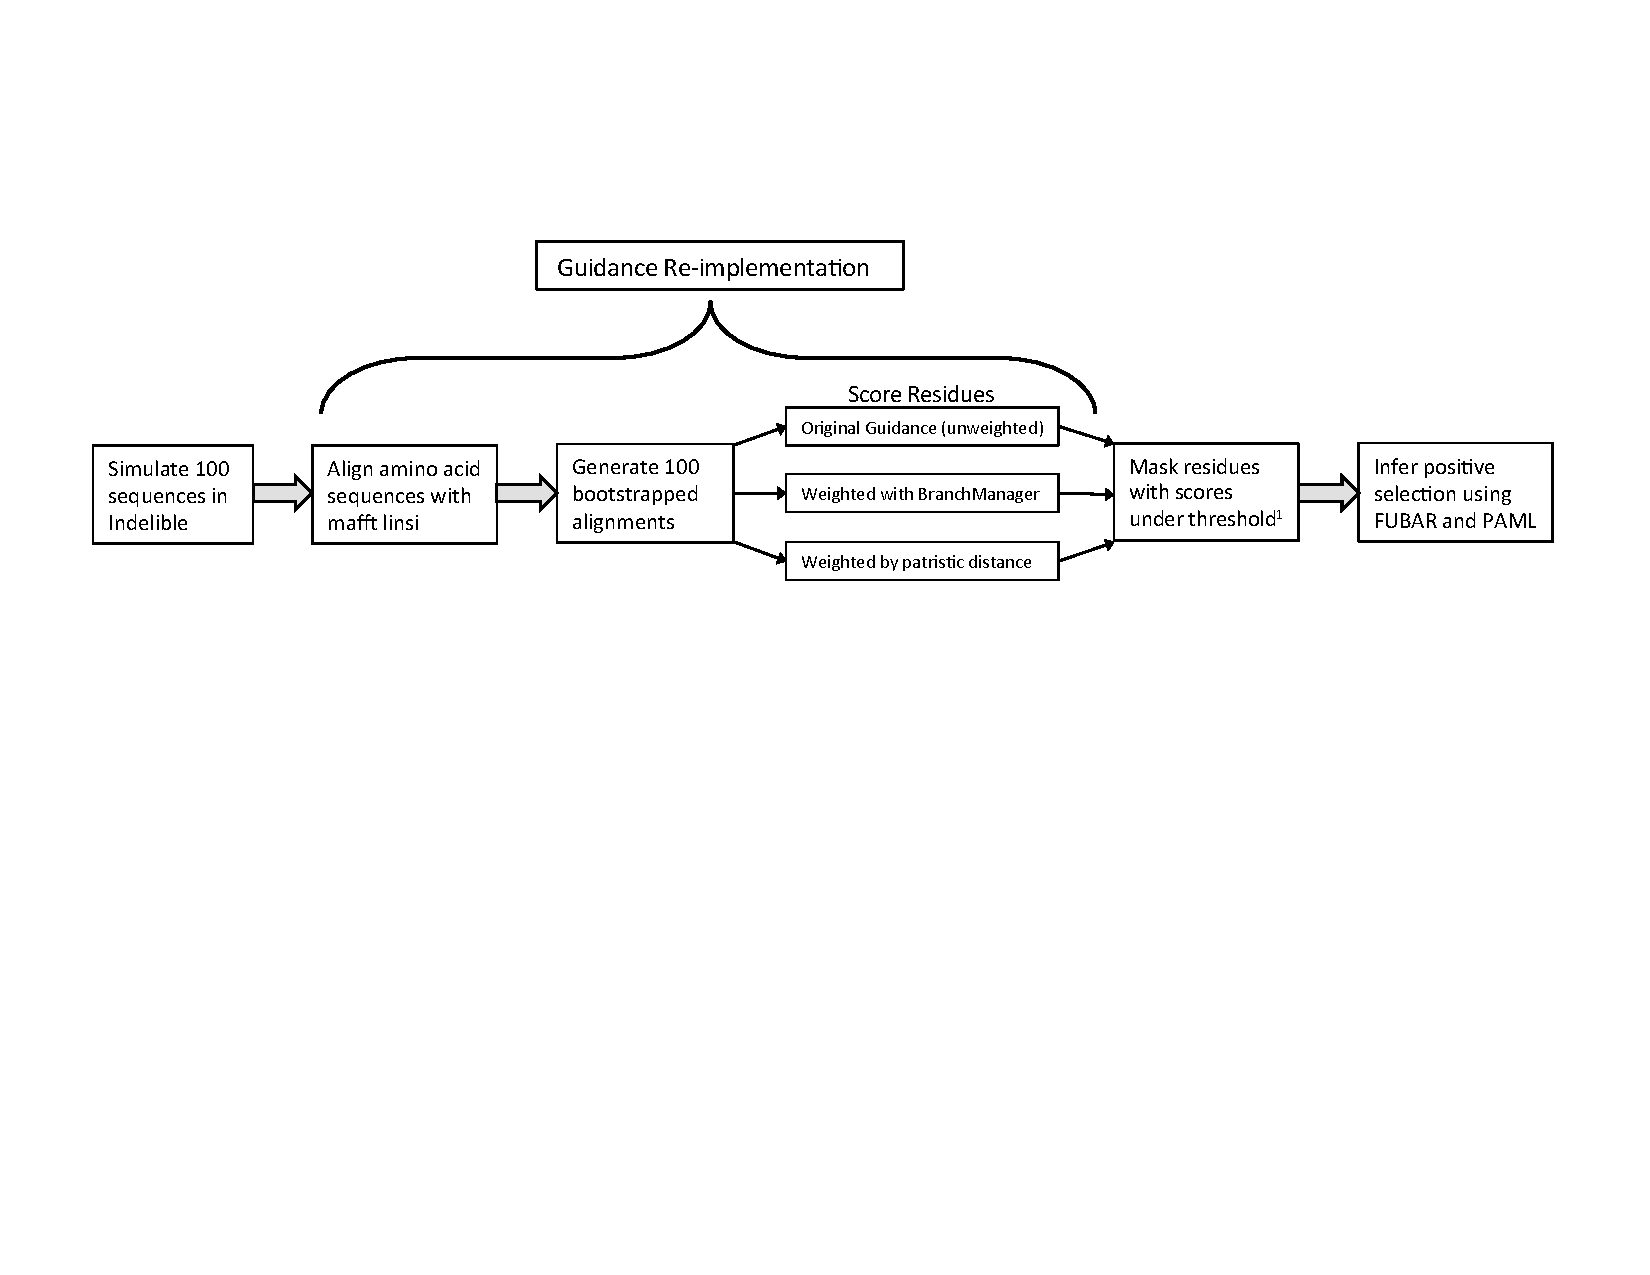
\includegraphics[width=7.5in]{Figures/pipeline.pdf}}
%\caption{Caption. I think you recommended less text in the pipeline figure, too. I'll work on that.}
%\label{pipeline} 
%\end{figure*}

%\begin{figure*}[H]
%\centerline{\includegraphics[width=7in]{Figures/roc_1_12_14.pdf}}
%\caption{A caption! Left: Fubar and Paml, full curves. Middle: Paml with Fubar greyed out. Right: Fubar with Paml greyed out. Only the gap-penalization algorithms are shown. Red=guidancep, blue=bmweightsp, yellow=pdweightsp.}
%\label{ROCcurves} 
%\end{figure*}


\begin{table}[H]
\label{tab:casemodel}
\caption {Effect of alignment filtering on the true positive rate of positive selection inference.}
\begin{tabular}{c l l l l l}
\hline\noalign{\smallskip}
Simulation Set & Method & Unfiltered & GuidanceP & BMweightsP & PDweightsP \\ 
\noalign{\smallskip}\hline\noalign{\smallskip}
11 taxa  & Fubar & 0.108 & 0.109   & 0.110   & 0.110        \\
              & Paml &  0.0873 & 0.0878       &  0.0881        & 0.0880 \\
\hline
26 taxa   & Fubar &  0.229 & 0.232       & 0.233 & 0.233         \\
              & Paml & 0.194 &\textbf{0.204}$^{\ast}$ &\textbf{0.203}$^{\ast}$ & \textbf{0.203}$^{\ast}$   \\
\hline
60 taxa  & Fubar & 0.345 & \textbf{0.379}$^{\ast\ast}$ & \textbf{0.377}$^{\ast\ast}$ & \textbf{0.375}$^{\ast\ast}$  \\
              & Paml & 0.447 & 0.447 & 0.440 & 0.445  \\
\hline
158 taxa & Fubar & 0.374 & \textbf{0.388}$^{\ast\ast}$ & \textbf{0.387}$^{\ast\ast}$ & \textbf{0.387}$^{\ast\ast}$  \\
\hline
\end{tabular}
\newline
\textsc{note.}--- Significance levels: $^{\ast\ast} P < 1\times10^{-5}$; $^{\ast} P < 1\times10^{-4}$. \textit{Unfiltered}: average true positive rate (TPR) for unfiltered alignments; \textit{GuidanceP}: average true positive rate (TPR) for alignments filtered with GuidanceP algorithm; \textit{BMweightsP}: average TPR for alignments filtered with BMweightsP algorithm; \textit{PDweightsP}: average TPR for alignments filtered with PDweightsP algorithm. All significance levels are relative to the given simulation set's unfiltered alignment. We detected no significant TPR differences among filters tested within sequence simulation sets. All significance levels were corrected for multiple comparisons with the single-step method.
\end{table}



\begin{table}[H]
\label{tab:penalmodel}
\caption {Comparison of gap-penalization vs original normalization schemes on the true positive rate of positive selection inference.}
\begin{tabular}{l l l}
\hline\noalign{\smallskip}
Simulation Set & Method & \textit{d} \\
\noalign{\smallskip}\hline\noalign{\smallskip}
11 taxa  & Fubar & 0.0007 \\
              & Paml & -0.0005\\
\hline
26 taxa   & Fubar & \textbf{0.0018}$^{\ast}$\\
              & Paml & \textbf{0.0061}$^{\ast\ast}$\\
\hline
60 taxa  & Fubar & \textbf{0.0089}$^{\ast\ast}$ \\
              & Paml & 0.0054  \\
\hline
158 taxa & Fubar & \textbf{0.002}$^{\ast\ast}$  \\
\hline
\end{tabular}
\newline
\textsc{note.}--- Significance levels: $^{\ast\ast} P < 1\times10^{-6}$; $^{\ast} P < 0.05$. \textit{d}: Magnitude of TPR difference between normalization schemes, represented as gap-penalization minus original. All significance levels were corrected for multiple comparisons with the single-step method.
\end{table}





\bibliographystyle{MBE}
\bibliography{citations}	

\end{document}